% !TEX TS-program = pdflatex
% !TEX encoding = UTF-8 Unicode
% !TEX ROOT = main.tex

\newpage
\section[Handzeichen]{Handzeichen für das Plenum}

\def\breite{5cm}
\def\ueberhang{0pt}
\begin{wrapfigure}{l}[\ueberhang]{0pt}
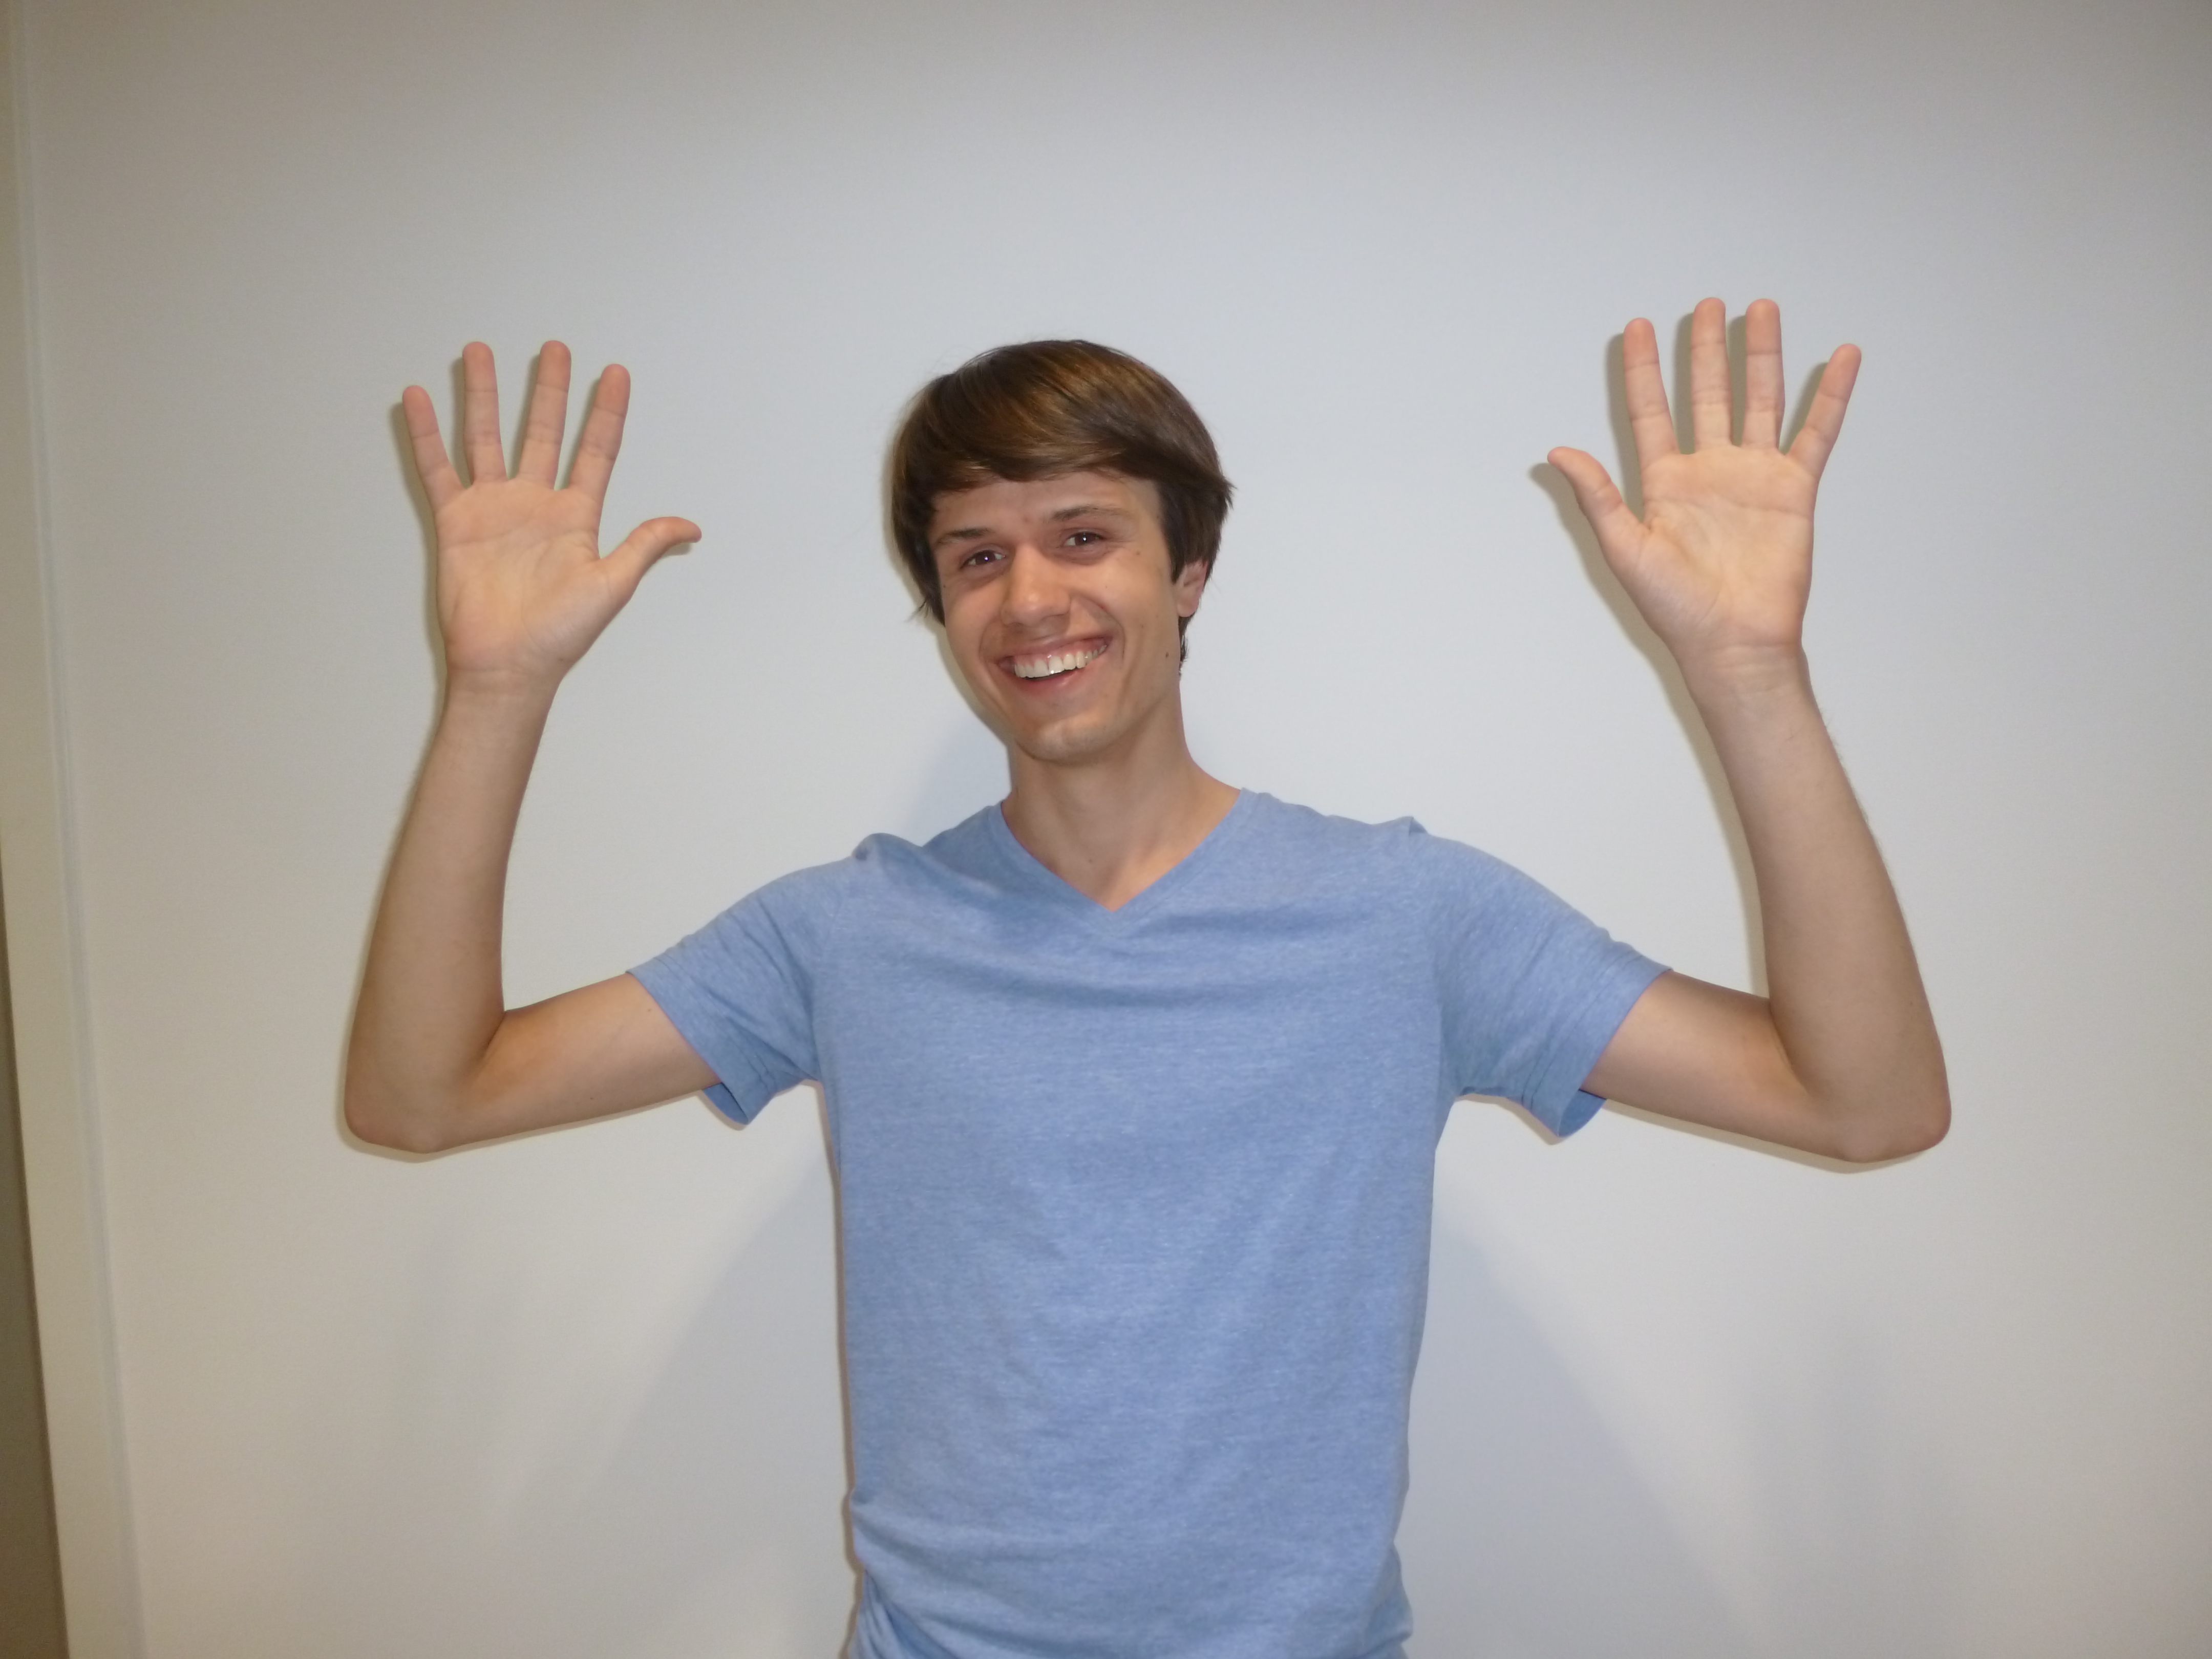
\includegraphics[width=\breite]{media/zustimmung}
\end{wrapfigure}

\subsection*{Zustimmung}
Kann -- ohne die sprechende Person zu unterbrechen -- durch Hände wedeln geäußert werden, genau so wie in der Gebärdensprache üblich. \\
\vspace{1cm}

\begin{wrapfigure}{l}[\ueberhang]{0pt}
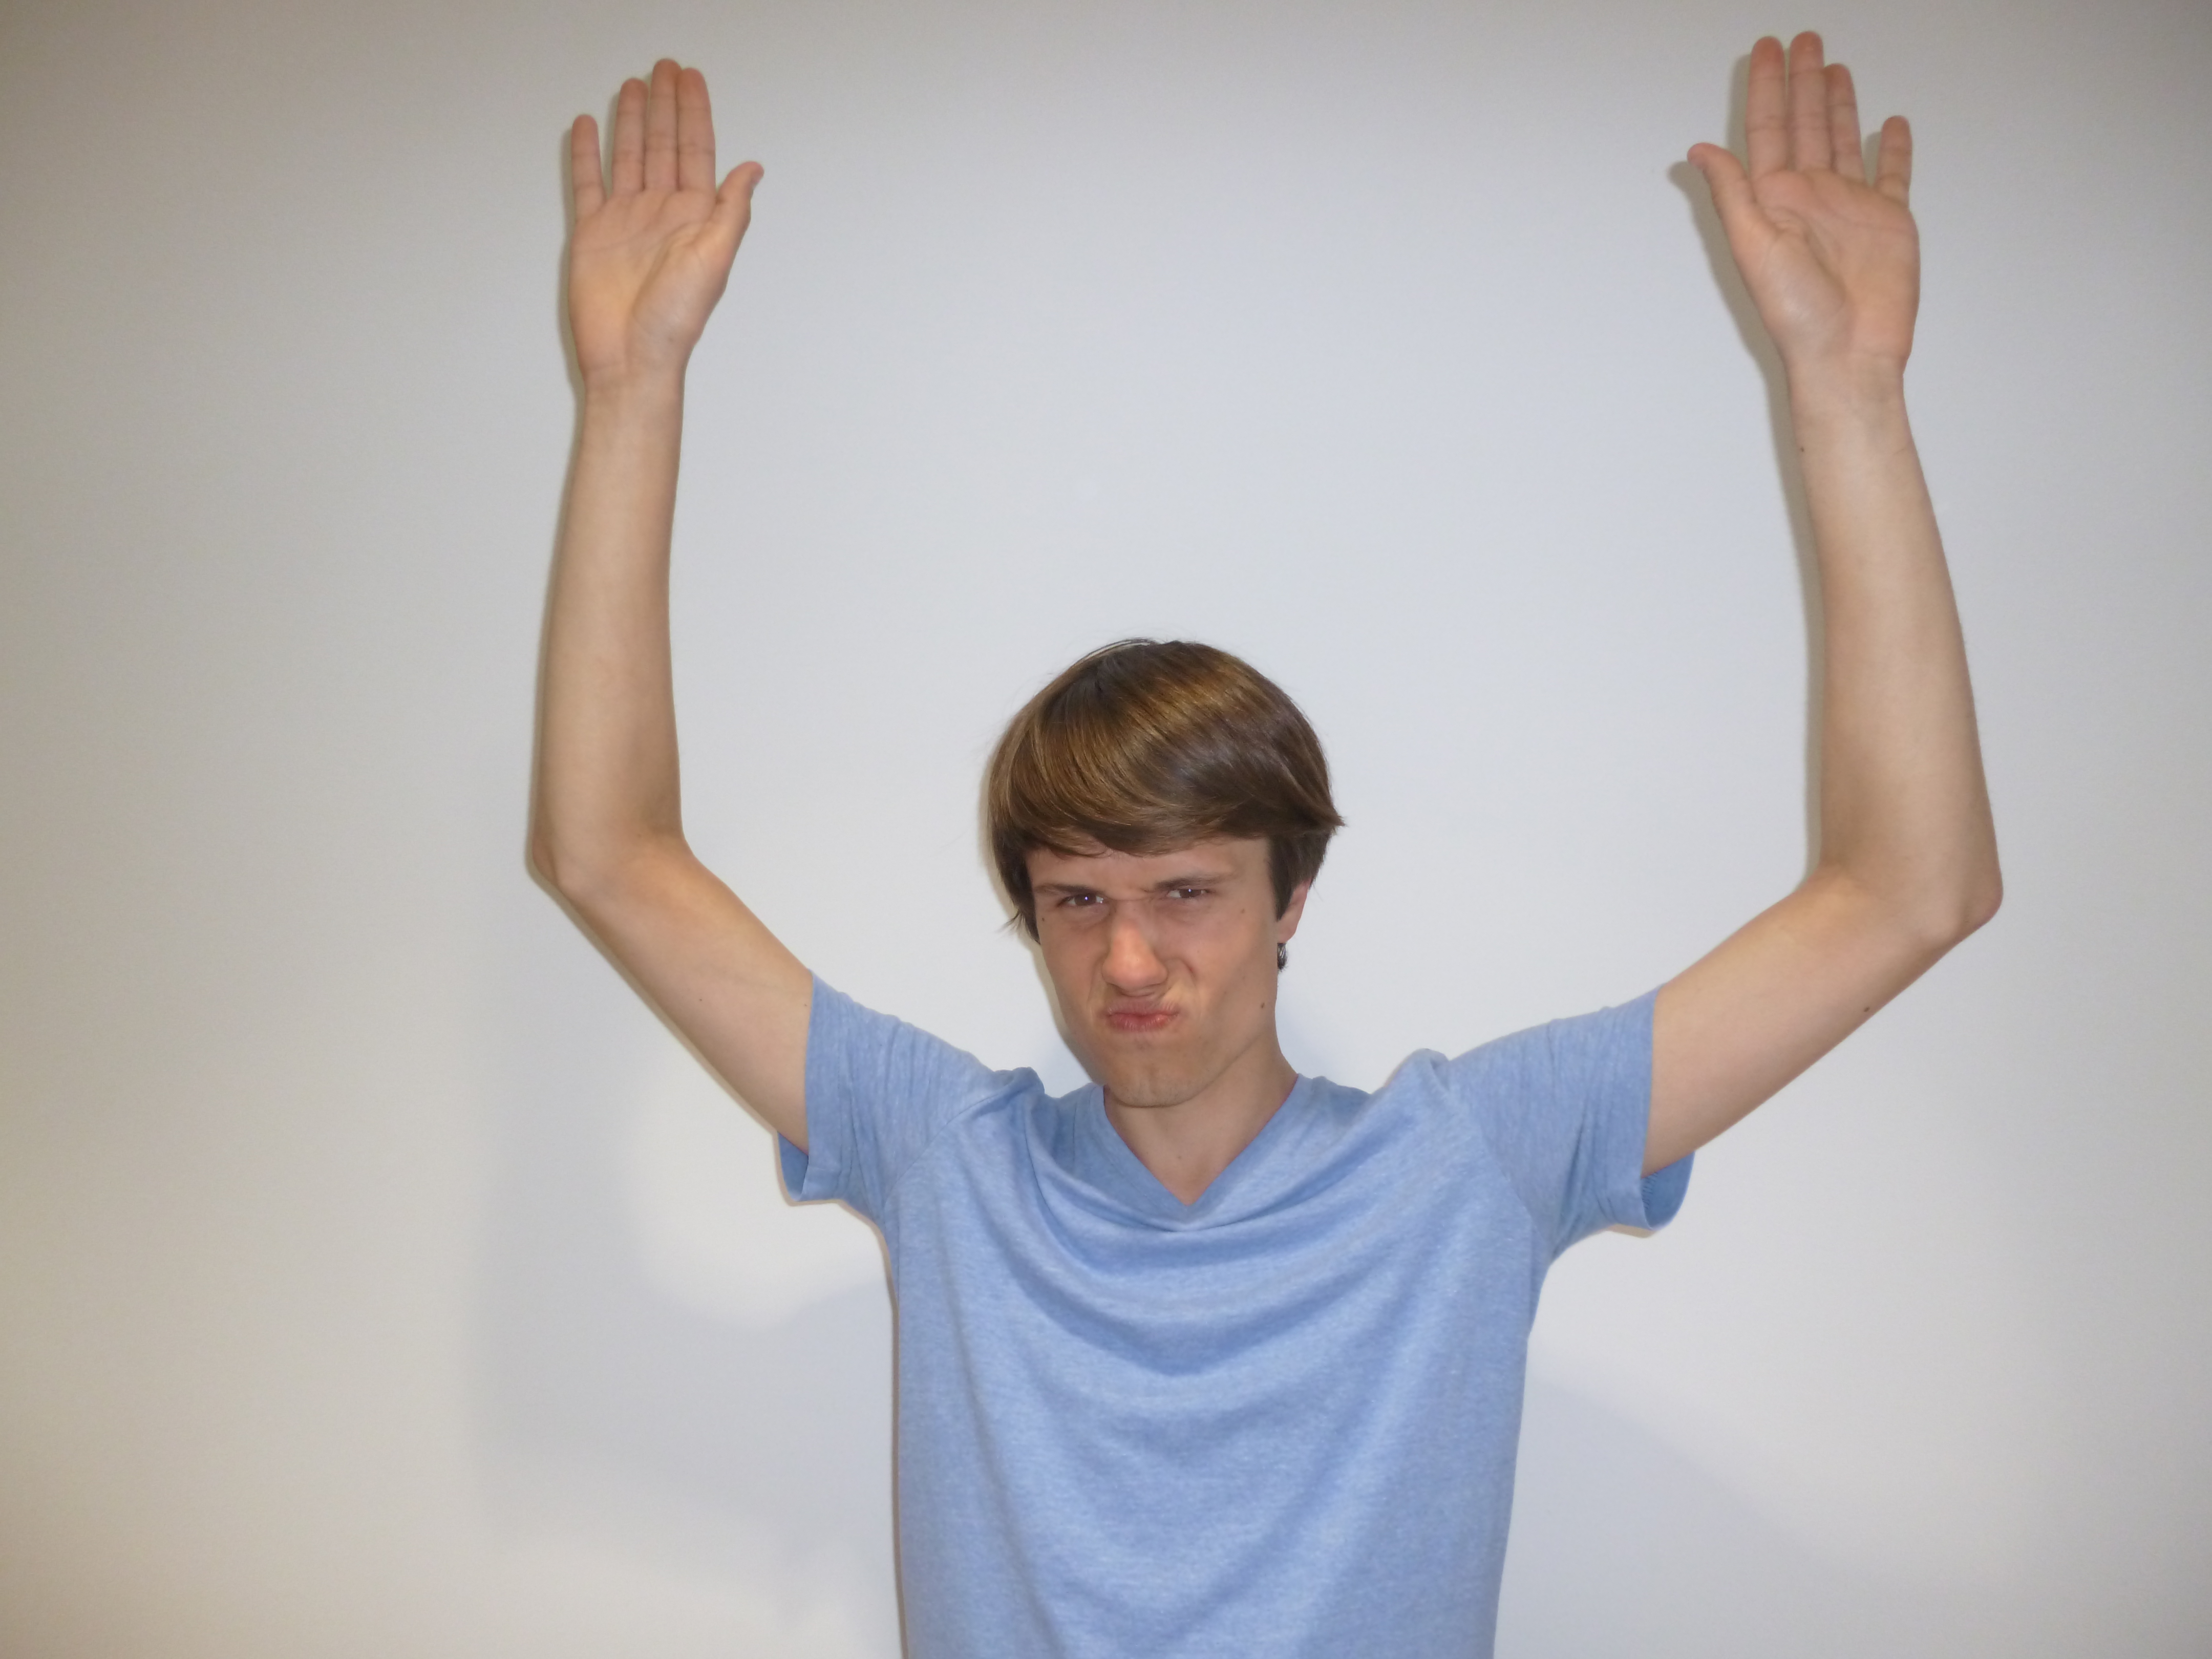
\includegraphics[width=\breite]{media/goantrag}
\end{wrapfigure}

\subsection*{GO-Antrag}
Beide Hände in die Höhe gestreckt zeigen einen GO-Antrag (s. \nameref{sec:go}) an, der gegenüber Redebeiträgen bevorzugt wird. Diese Anträge sollen auf konstruktive Weise die Debatte oder Entscheidungsfindung unterstützen.

\begin{wrapfigure}{l}[\ueberhang]{0pt}
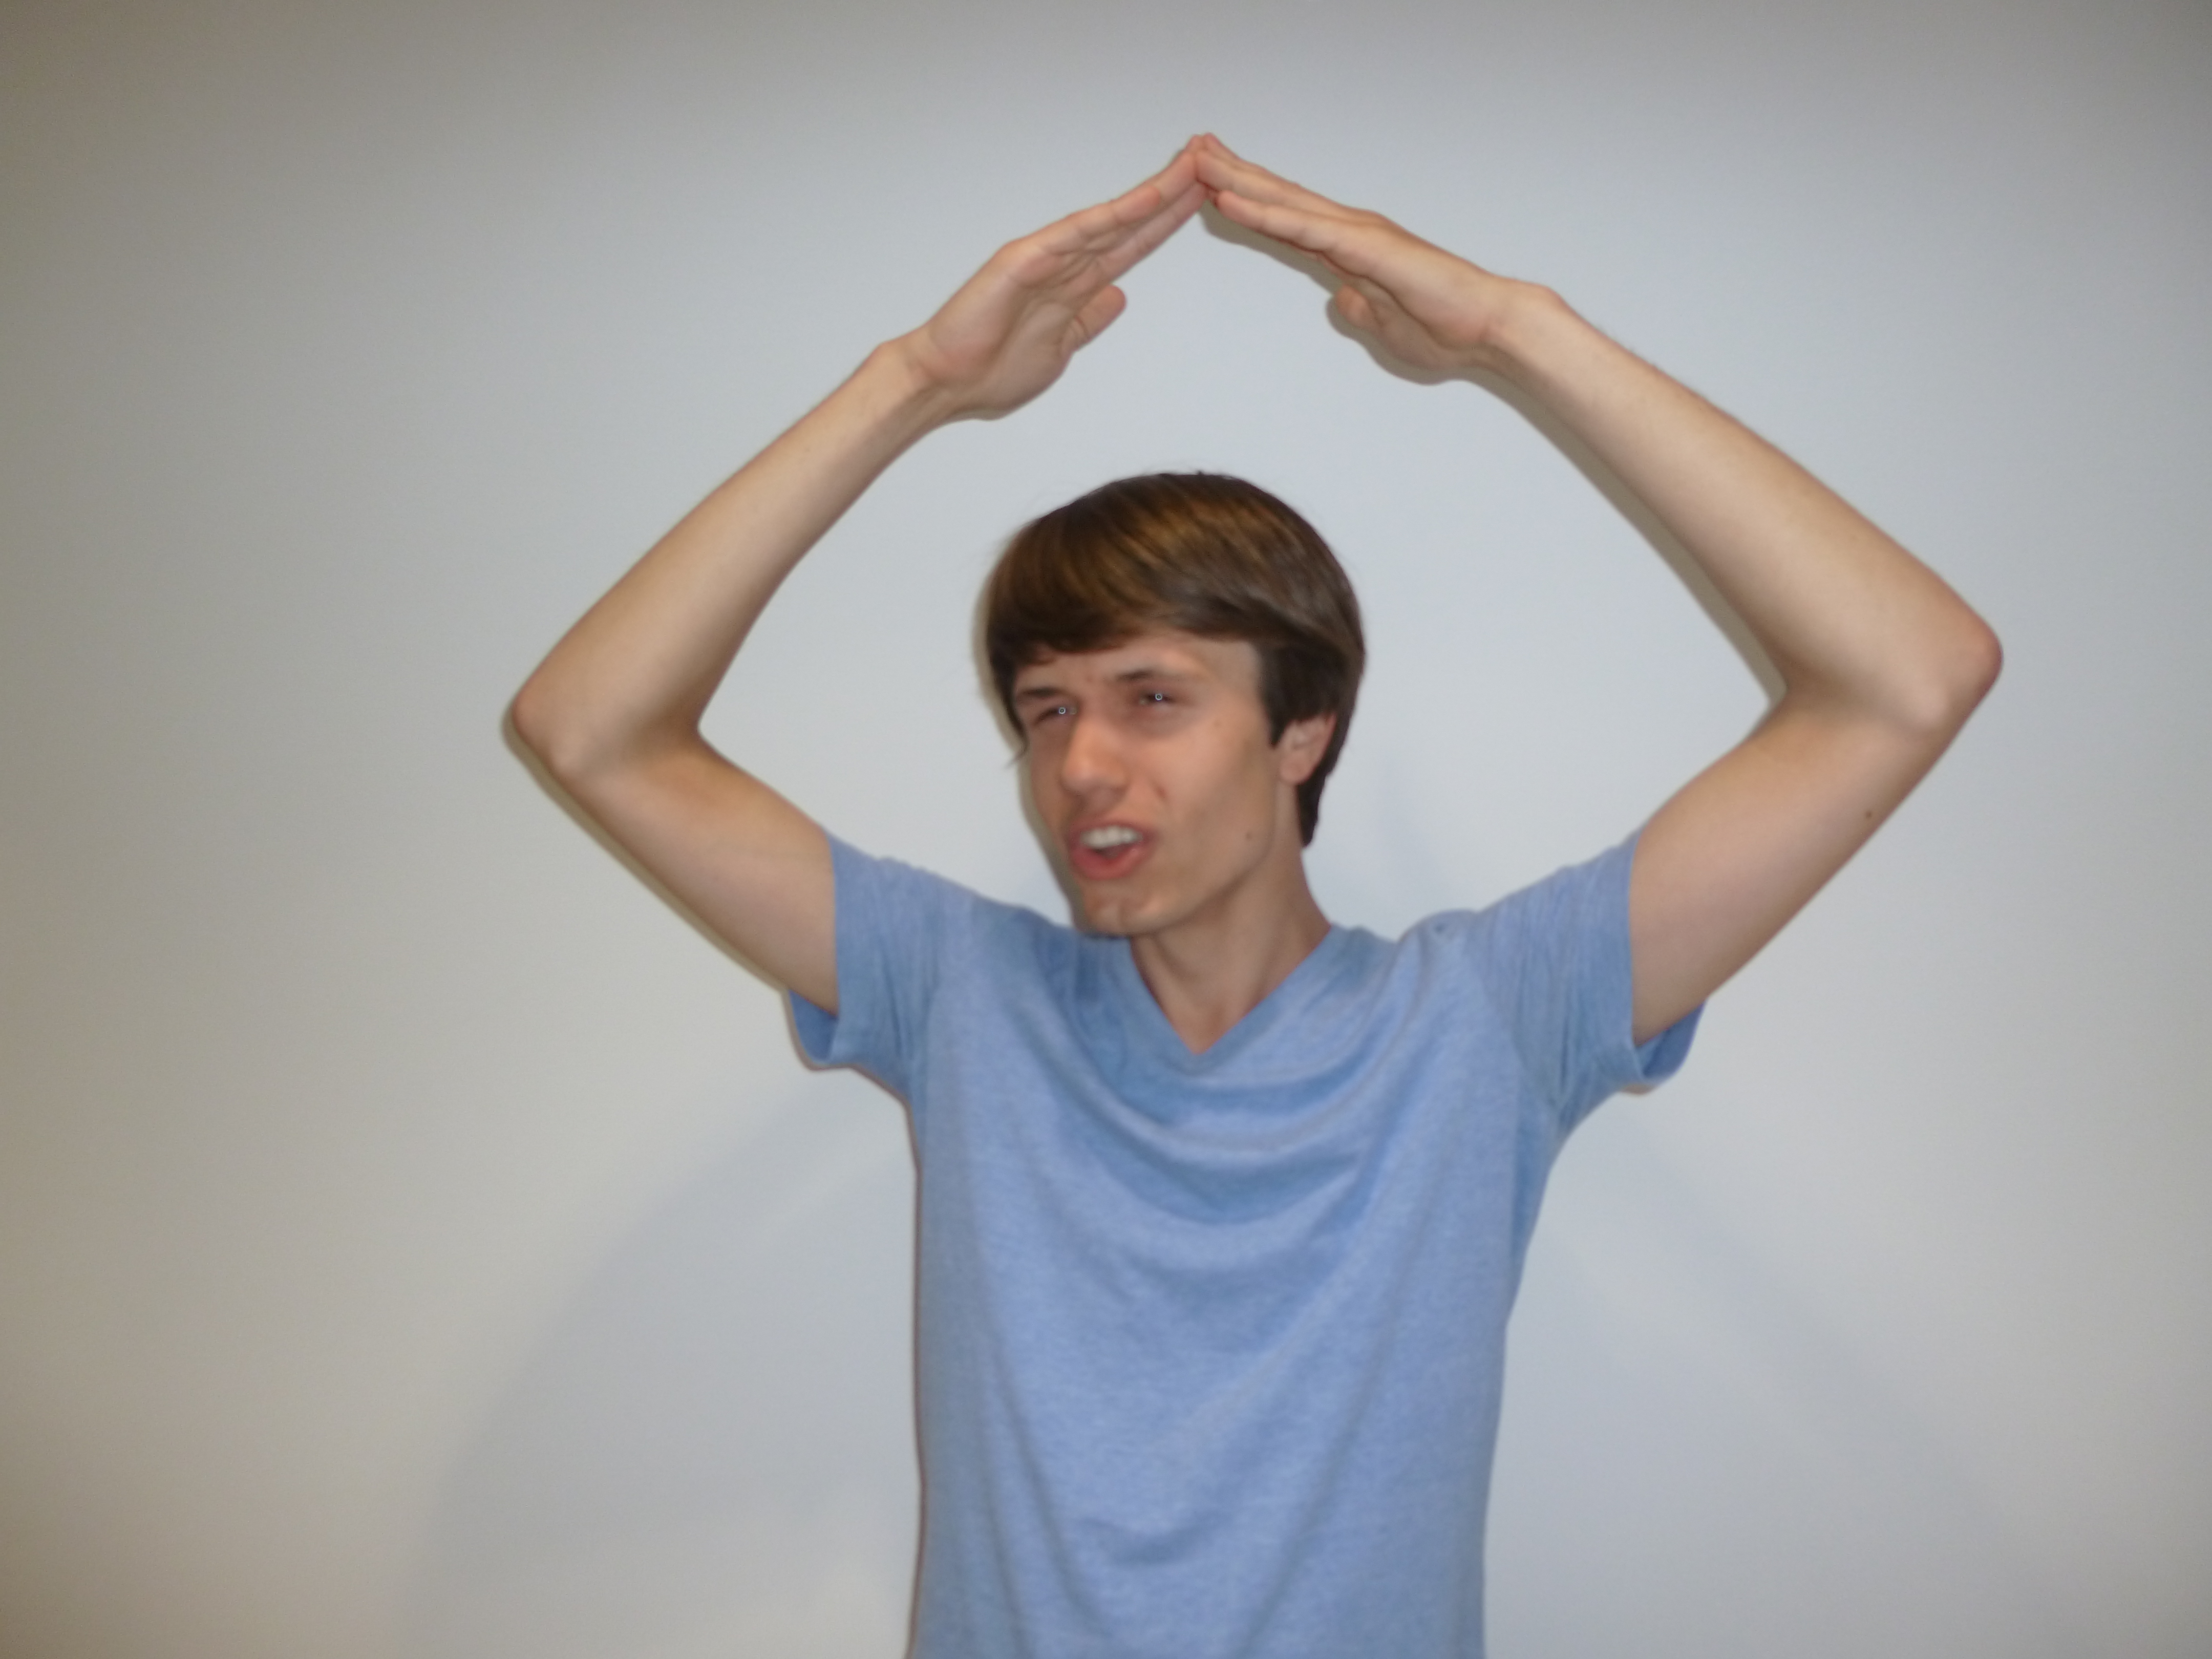
\includegraphics[width=\breite]{media/nachfrage}
\end{wrapfigure}

\subsection*{Inhaltliche Nachfrage}
Ein durch Arme und Hände geformtes Dreieck über den Kopf zeigt eine inhaltliche Nachfrage an. Diese kann gestellt werden, wenn Begrifflichkeiten oder Vorgänge unklar sind, z.\,B. eine unbekannte Abkürzung verwendet wurde oder der Abstimmungsmechanismus unzureichend erklärt wurde.